\documentclass{article}
\usepackage[T1]{fontenc}
\usepackage{lmodern}
\usepackage{graphicx}
\usepackage{amsmath,amssymb}
\usepackage[a4paper,margin=2cm]{geometry}
\usepackage[absolute,overlay]{textpos}
\setlength{\TPHorizModule}{1mm}
\setlength{\TPVertModule}{1mm}
\usepackage[indonesian]{babel}
\usepackage{hyperref}
\setlength{\emergencystretch}{2em}
% unit: Halaman 21

\begin{document}

% === Halaman 21 (python/native) ===

Transformasi ShiftRows()

• Transformasi ShiftRows() melakukan operasi permutasi dengan pergeseran secara 

wrapping (siklik) pada 3 baris terakhir array state. 

• Jumlah pergeseran bergantung pada nilai baris (r). Baris r = 1 digeser sejauh 1 byte, 

baris r = 2 sejauh 2 byte, dan baris r = 3 sejauh 3 byte. Baris r = 0 tidak digeser.

% deskripsi: gambar native xref 136
\noindent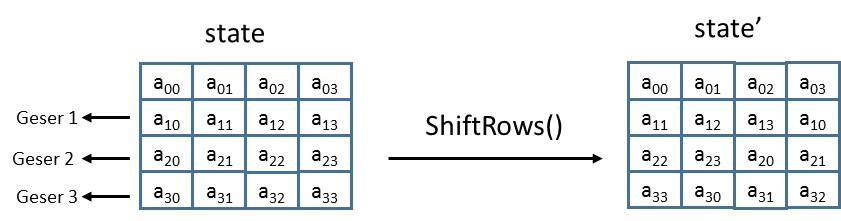
\includegraphics[width=0.85\textwidth]{../../images/python/page_021_img_01.jpeg}

\end{document}
